\section{Physical Scheduler Results}
\subsection{Primary Attribution and Robustness}
All forty primary runs contain 501 power samples and 500 decisions. Relative to Static-MedRF, Tabular-Q saves \TQSavingJ{} J (95\% paired CI \TQSavingJLow{}--\TQSavingJHigh{}) and DQN saves \DQSavingJ{} J (\DQSavingJLow{}--\DQSavingJHigh{}), but both lose \TQFOneDropPP{} F1 pp and \TQRecallDropPP{} recall pp. Both select LightLR in all 5,000 windows; thus the result does not demonstrate switching.

The matched Static-LightLR control directly compares the learned policies with Static-LightLR. Tabular-Q has identical predictions and +0.455 J with CI $[-1.861,2.772]$ J; DQN has identical predictions and +4.525 J [2.693,6.357]. The isolated state-to-action benchmark time is 10.8~$\mu$s for Tabular-Q and 1.567 ms for DQN, but timing is not converted into joules. Twenty policy seeds, 85 reward/state runs, and 35 Tabular-Q $\alpha/\gamma$ runs remain single-action on held-out support; only the detection-only objective selects MedRF rather than LightLR. Full primary and strengthening tables are supplementary.

\subsection{Fixed-Rate Confidence Cascade}
Table~\ref{tab:r1} reports ten new matched blocks. The fixed cascade escalates 1.34\% of rows and raises F1 by 1.347 pp versus Static-LightLR while using +7.952 J [5.897,10.007]. Its raw mean-power difference is +15.917 mW [11.798,20.035], whereas preceding-idle adjustment gives +13.635 mW $[-1.515,28.784]$; environmental drift therefore weakens the power attribution but not the raw-energy result. Cascade F1 (0.98391) is close to Static-MedRF (0.98386), with 0.279 lower recall pp and 0.156 lower FPR pp.

The cascade latency is implementation- and call-granularity-specific. Frozen executed source first runs LightLR on the full 100-row batch and, when needed, makes \emph{one} MedRF call on the deferred sub-batch; it does not call MedRF once per deferred row. Although only 1.3388\% of rows are deferred, they are spread across 3,338/5,000 windows (66.76\%), with only 2.01 deferred rows per active window. Windows without escalation average 1.636 ms, whereas escalation-active windows average 31.884 ms, close to the cost of one MedRF call; the resulting overall cascade mean is 21.830 ms. Thus This campaign measures this 100-row, small-sub-batch implementation regime and is not a general energy or latency bound for optimized cascade systems.

\begin{table*}[t]
\centering\footnotesize
\caption{Fixed-rate cascade physical results; means over ten paired blocks. Adjusted power subtracts the immediately preceding idle. Escalation is the fraction sent from LightLR to MedRF.}
\label{tab:r1}
\setlength{\tabcolsep}{4.0pt}
\begin{tabular}{lrrrrrrr}\toprule
Method & Energy (J) & Power (W) & Adjusted (mW) & F1 & Recall (\%) & FPR (\%) & Escalation (\%)\\\midrule
\tableinput{tables/r1_revision_rows}
\bottomrule\end{tabular}
\end{table*}

\subsection{Variable Load, Feasibility, and State Coverage}
The variable-load campaign visits all nine frozen load/prevalence cells in every run. DeadlineGuard executes MedRF in 3,500 and LightLR in 1,500 of its 5,000 windows, with 5.3 recorded switches/run, and misses no service deadline. Static-MedRF misses 512/5,000 deadlines (10.24\%, block CI 9.32--11.16\%) although its final backlog returns to zero. Cascade misses 21/5,000; all other methods miss none.

The strongest paired comparison is DeadlineGuard against Static-MedRF. DeadlineGuard uses 43.714 J less per run (95\% paired CI 41.418--46.010 J), a 2.98\% reduction relative to the 1468.1-J Static-MedRF mean, while reducing the deadline-miss rate by 10.24 pp to zero. The trade-off is 1.373 pp lower F1 and 2.853 pp lower recall. All ten energy differences have the same direction (exact sign-flip $p=0.00195$). This establishes a measured feasibility/energy benefit for the simple causal rule relative to the high-security static baseline, not universal superiority over all static choices.

The frozen learned policies do not provide useful load adaptation. DQN remains LightLR in all 5,000 windows and reproduces its detection. Tabular-Q reaches new load-related states and selects TinyDT in every window through the frozen tabular default, yielding F1 0.7434 with FPR 67.76\%. Here ``fallback'' is registry terminology, not an exception branch. On unseen zero-initialized rows, \texttt{np.argmax} returns the first maximum and the configured action order places TinyDT first. Thus the variable-load failure is the hardware realization of the off-support tie behavior already visible in the 314/324-state TinyDT greedy map.

The fixed heuristic provides a switching contrast rather than a no-op baseline. CFSM averages 9.8 switches per run, but spends 74.20\% of windows on TinyDT and only 22.26\% on HeavyMLP (LightLR 2.28\%, MedRF 1.26\%). Its switching changes detector identity without reaching a reliable security operating point; the low F1 is not evidence that CFSM simply selected one static model.

Variable-load raw energy is heterogeneous across methods, so Table~\ref{tab:r2} now reports run SDs and selected paired contrasts are separated in Table~\ref{tab:r2pairs}. For DQN versus Static-LightLR, all ten raw block differences are positive (median +5.72 J; exact sign-flip $p=0.00195$), but one Block~4 excursion is +392.0 J and inflates the SD of differences to 122.2 J, giving a Student-$t$ interval of $[-43.2,131.7]$ J. That run coincides with a 3.919-W preceding idle and a 49.2$^\circ$C maximum temperature, unlike the other DQN blocks; idle-adjusted power does not resolve a DQN--LightLR difference. We therefore report a consistent raw direction but an unstable magnitude and make no controller-power attribution because the controller-only power arm was not executed.

For scale only, the isolated DQN state-to-action timing is 1.5669~ms. Five thousand decisions therefore amount to 7.8345~s of controller CPU time. If an external device-power increment were hypothetically 0.2, 0.5, or 1.0~W, the corresponding upper-bound contributions would be 1.57, 3.92, and 7.83~J, respectively. These are sensitivity calculations, not measurements: no controller-power increment was measured and none is used to attribute the physical DQN premium.

DeadlineGuard uses +7.550 J [5.033,10.068] and +14.160 adjusted mW [0.374,27.947] relative to Static-LightLR. Static-MedRF uses +51.264 J [49.537,52.991] and +98.609 adjusted mW [79.296,117.922] relative to LightLR. Cascade improves F1 by 1.384 pp but its raw +31.262 J interval crosses zero; the idle-adjusted +98.843 mW interval [77.885,119.802] does not. Raw and preceding-idle-adjusted endpoints are retained separately because they answer different questions.

\begin{table*}[t]
\centering\footnotesize
\caption{Variable-load results over ten paired blocks. Energy is mean$\pm$SD across runs; deadline miss is the fraction of one-second windows missing the service deadline.}
\label{tab:r2}
\setlength{\tabcolsep}{3.1pt}
\begin{tabular}{lrrrrrrr}\toprule
Method & Energy (J) & Power (W) & F1 & Recall (\%) & FPR (\%) & Miss (\%) & Completion p95 (s)\\\midrule
\tableinput{tables/r2_revision_rows}
\bottomrule\end{tabular}
\end{table*}

\begin{table}[t]
\centering\scriptsize
\caption{Selected variable-load paired contrasts, $n=10$ blocks. $\Delta E$ is first method minus second; detection and deadline changes are percentage points.}
\label{tab:r2pairs}
\resizebox{\columnwidth}{!}{%
\begin{tabular}{lrrrr}\toprule
Contrast & $\Delta E$ (J), 95\% CI & $\Delta$F1 & $\Delta$Miss & sign-flip $p$\\\midrule
\tableinput{tables/r2_key_paired_rows}
\bottomrule\end{tabular}}
\end{table}

\begin{figure}[t]
\centering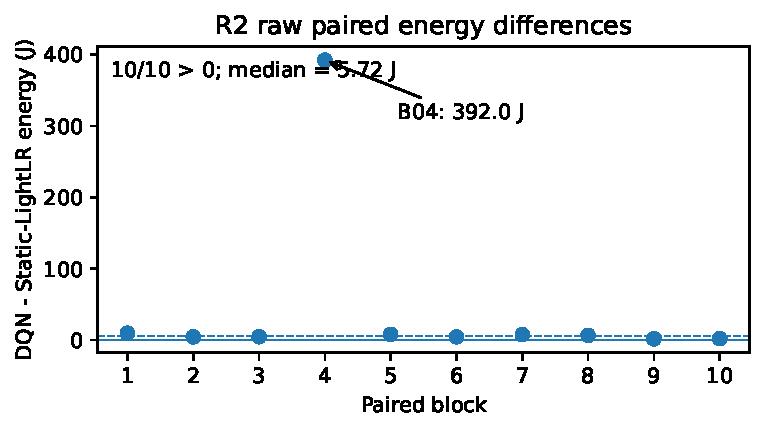
\includegraphics[width=\columnwidth]{figures/r2_dqn_block_energy_differences.pdf}
\caption{Raw DQN-minus-Static-LightLR energy difference for each paired block. All ten are positive, but Block~4 is a large power/temperature excursion; the dashed line is the median (5.72 J).}
\label{fig:r2dqnblocks}
\end{figure}

\begin{figure}[t]
\centering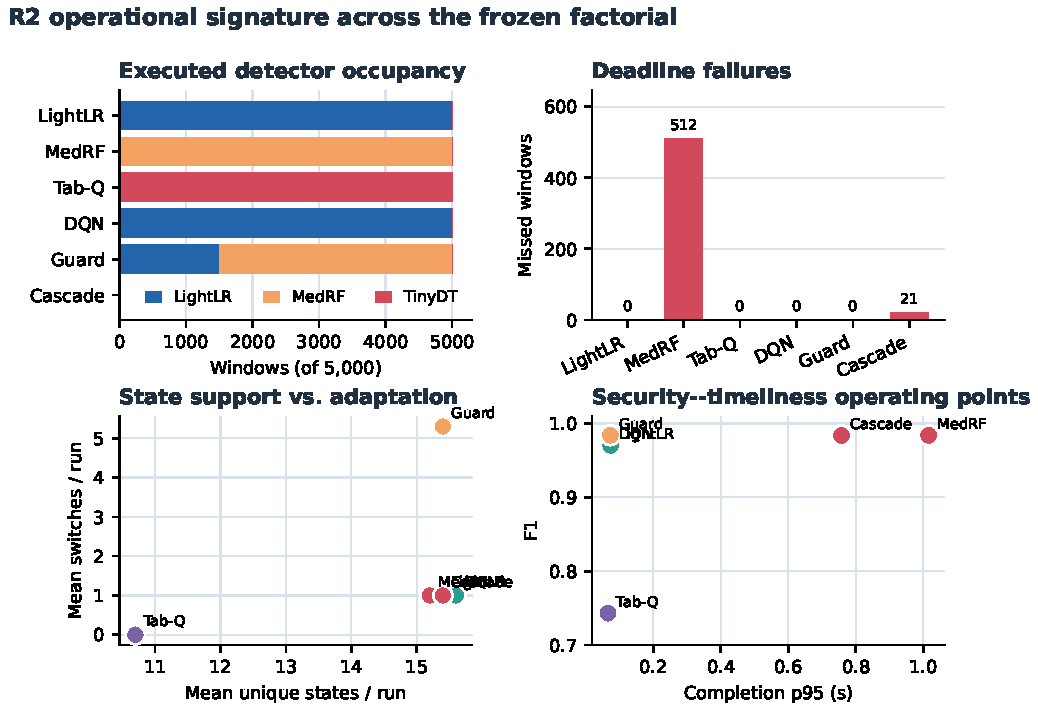
\includegraphics[width=\columnwidth]{figures/r2_operational_dashboard.pdf}
\caption{Variable-load operational dashboard: realized detector occupancy, deadline misses, state support/switching, and security--timeliness operating points in the same frozen 60-run factorial.}
\label{fig:r2dashboard}
\end{figure}

\subsection{Protocol Stop and TinyDT Threshold Diagnostic}
The planned controller-only power arm is not missing data: it is a protocol-preserving stop. Its design required four original observed-support states, but the frozen registry exposes eight and supplies no pre-outcome selection rule. Choosing four afterward would modify the protocol, so no controller-only power segment was run and no DQN joule attribution is made.

The threshold diagnostic selects threshold 0.646751 on validation and applies it once to test. At threshold 0.5, TinyDT test F1/FPR/recall are 0.4792/67.78\%/99.76\%; the diagnostic yields 0.9698/1.82\%/99.61\%, with balanced accuracy 0.9889 and AUROC 0.9906. The large recovery with near-constant recall is consistent with a shifted decision threshold rather than absent ranking information. It does \emph{not} make TinyDT an acceptable substitute in the frozen physical study: every classifier and scheduler artifact in those campaigns was fixed at threshold 0.5, and the post-hoc threshold cannot retroactively rehabilitate the unsafe TinyDT actions. The diagnostic therefore explains calibration sensitivity without replacing any primary or physical result.

\begin{table}[t]
\centering\scriptsize
\caption{TON-IoT TinyDT test: fixed primary versus post-hoc validation-selected threshold.}
\label{tab:r4}
\setlength{\tabcolsep}{2.1pt}
\resizebox{\columnwidth}{!}{%
\begin{tabular}{lrrrrrrrrr}\toprule
Result & $\tau$ & TN & FP & FN & TP & F1 & Rec. & FPR & BA\\\midrule
\tableinput{tables/r4_threshold_rows}
\bottomrule\end{tabular}}
\end{table}

The same validation-only procedure was also applied offline to the other frozen TON-IoT detector scores. Table~\ref{tab:allthreshold} shows the resulting test diagnostics; no detector was retrained and no physical campaign was changed. TinyDT is the clear F1/FPR outlier: its validation-selected threshold changes test F1 by +49.05 points, whereas the other detectors change by at most 0.29 points. This separates calibration sensitivity from the sparse-state and deterministic-tie mechanism.

\begin{table*}[t]
\centering
\footnotesize
\caption{Offline validation-selected threshold diagnostic for every frozen TON-IoT detector. The physical campaigns remain fixed at $\tau=0.5$.}
\label{tab:allthreshold}
\setlength{\tabcolsep}{4pt}
\begin{tabular}{lrrrrrrr}\toprule
Model & $\tau=0.5$ F1 & $\tau=0.5$ FPR (\%) & $\tau^\star$ & $\tau^\star$ F1 & $\tau^\star$ FPR (\%) & $\Delta$F1 (pp) & Validation BA\\\midrule
\tableinput{tables/all_detector_threshold_rows}
\bottomrule\end{tabular}
\end{table*}
